\textbf{Comparision of pressure between non-cavitating and cavitating flows over a suction side of hydrofoil}:
A better way to understand this concept is to compare the final time step of cavitation and non-cavitation flow. 
Figure(4.7) illustrates AOA $3.2^{\circ}$, which is a non-cavitating angle, in comparison to AOA $4.1^{\circ}$ and $8^{\circ}$, which show a cavitating angle. 
During cavitation, the cavitation zone pressure was equal to the vapor pressure. As a result of the cavitation effect, 
the pressure distribution over the suction side of the membrane was greatly impacted, and the pressure gradient across 
the membrane cavity at the closure was  greater than in the absence of cavitation. However, the change on the 
pressure side of the foil was much smaller. The other angles of attack in the table (4.8) and (4.9) show similar physics while 
comparing with the non-cavitating condition of pressure in figure(4.2). The change in pressure distribution also affected 
the overall hydrodynamic performance of the hydrofoil.
\begin{figure}[H]
    \centering
  \subfloat[$\alpha={{3.2}^{\circ}}$]{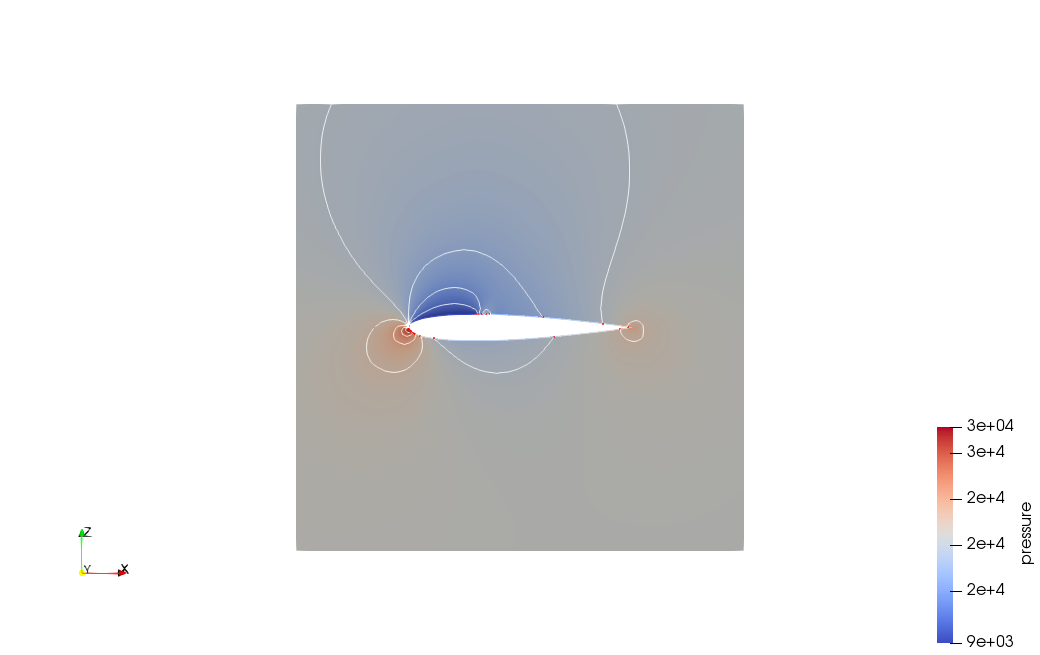
\includegraphics[width=0.3\textwidth]{AOA3.2pressurecontour}}
   \subfloat[$\alpha={{4.1}^{\circ}}$]{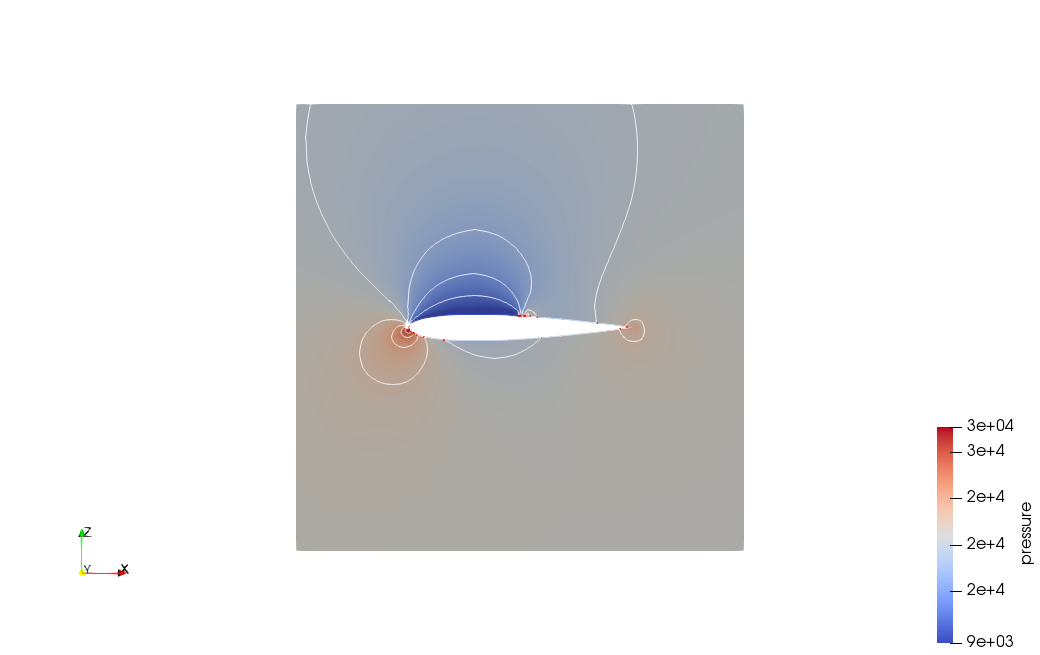
\includegraphics[width=0.3\textwidth]{AOA4.1pressurecontour}}
   \subfloat[$\alpha={{8}^{\circ}}$]{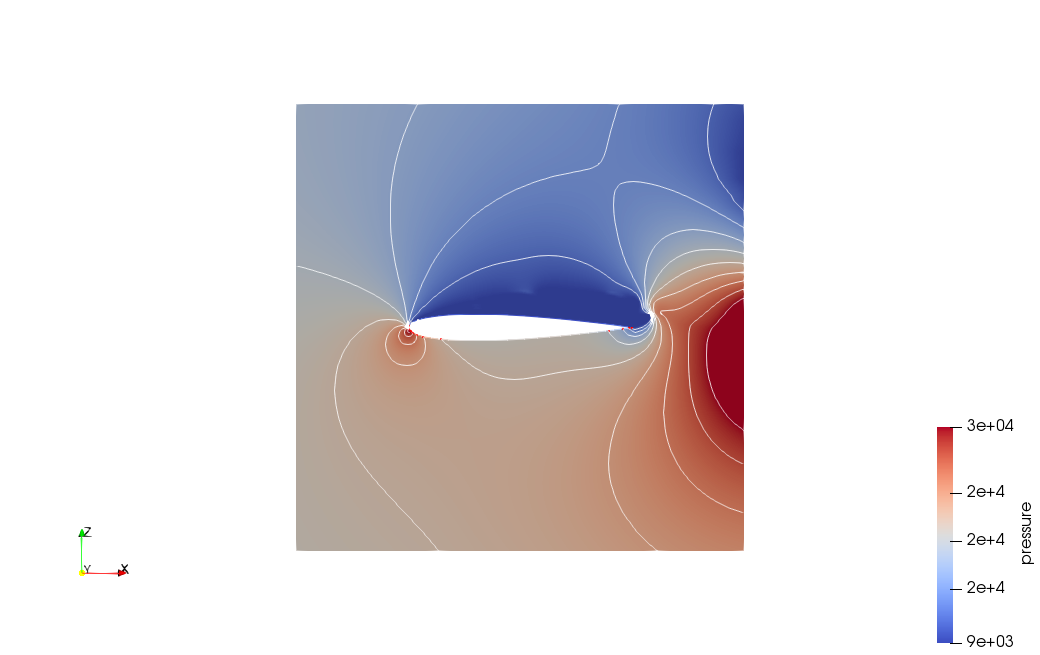
\includegraphics[width=0.3\textwidth]{AOA8pressurecontour}}
    \caption{Contrast between the pressure distribution of the cavitating and non-cavitating flows}
    \label{fig:fig16}
\end{figure}

As can be seen in figure (4.5), the length of the cavity based on the cavitation zone is equal to the vapor pressure 
on the suction side of the hydrofoil which increases as the angles of attack increase as can be seen in the table (4.8) and (4.9). 
The $C_p$vs x/c graph in the table (4.12) and (4.13) illustrates this phenomenon. The graph shows that, for an AOA of $4.1^{\circ}$ to $5.7^{\circ}$, 
there is a rise in pressure after $(1/4)^{th}$ of the chord of the suction side of the hydrofoil due to adverse pressure gradient.
In AOA $6.5^{\circ}$ to $8^{\circ}$, the length of the cavity is equal to the chord length of the hydrofoil. 
This means that the observed state completely covers the suction side of the hydrofoil with vapor. 
On the other hand, there is no pressure rise after  $(1/4)^{th}$ chord and  a transient state can be observed as can seen from the 
table(4.13). More often, these angles of attack are in the state of the stall, and there is a vortex rollup accompanied by 
a filled vapor state as can be seen from the table(4.6) and (4.7).

\textbf{3D simulation of  cavitation along spanwise  over a  NACA0012 at an angle of attack 8$^{\circ}$}
The extension of 2D to 3D is performed by using the 
\textit{blockMeshDict} file. In domain of the \textit{blockMeshDict} one should add $ymax = 0.45$ and $ymin =-0.45$ along the spanwise direction; due to this extension, 10 processor cores are used to simulate the 3D cavitation flows.
\begin{figure}[H]
    \centering
    \subfloat[t=0.5 s]{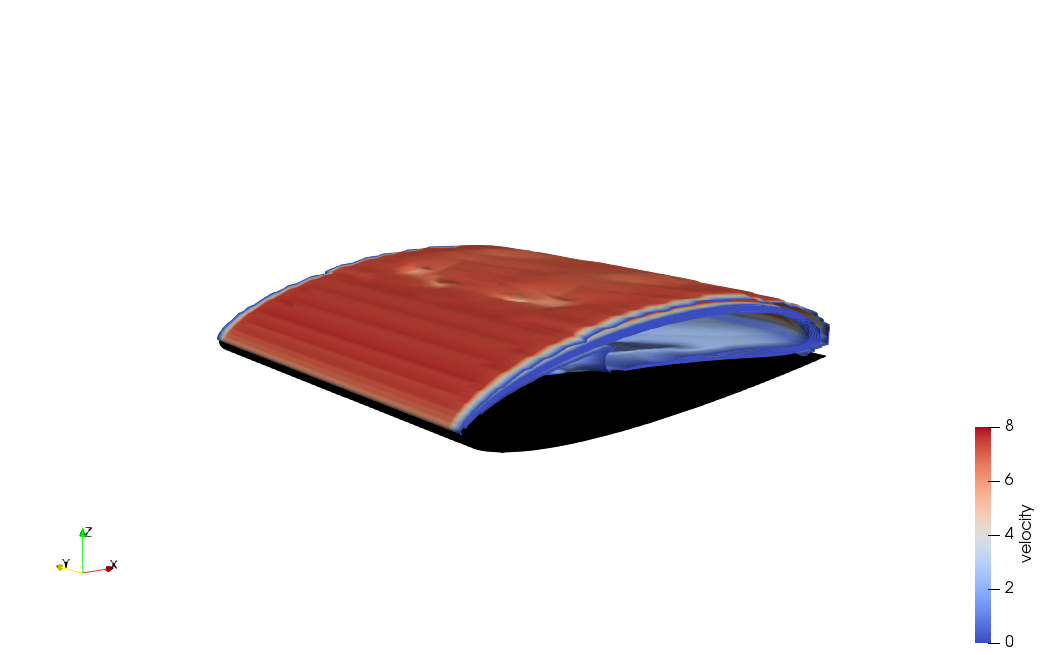
\includegraphics[width=0.3\textwidth]{AOA3Dt0.5v}}
    \qquad
  \subfloat[t=0.7 s]{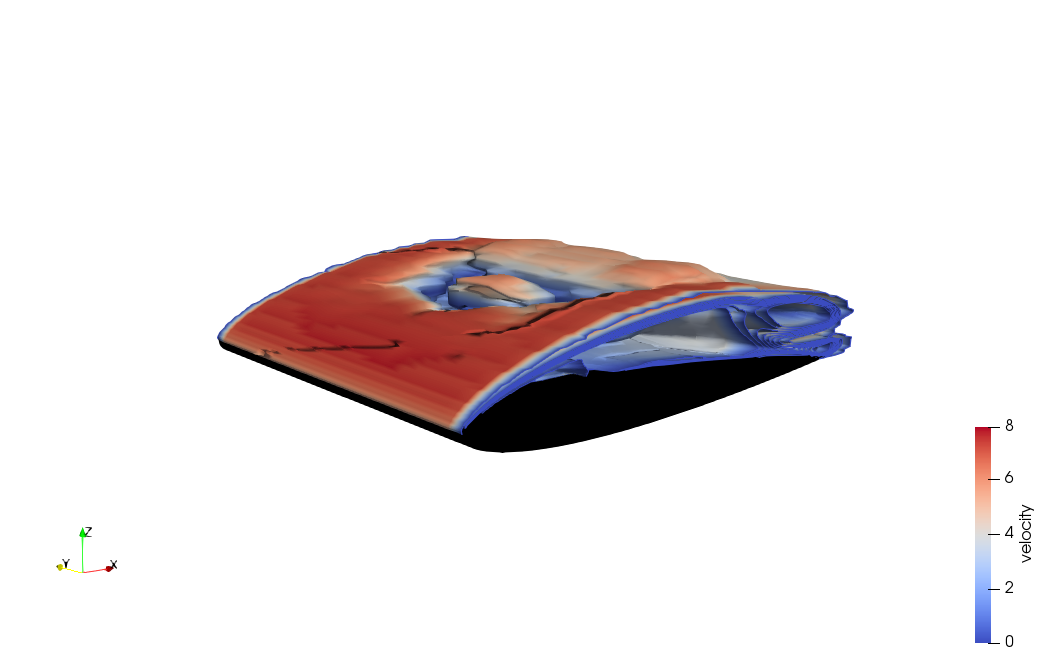
\includegraphics[width=0.3\textwidth]{AOA3Dt0.7v}}
   \qquad
  \subfloat[t=0.9 s]{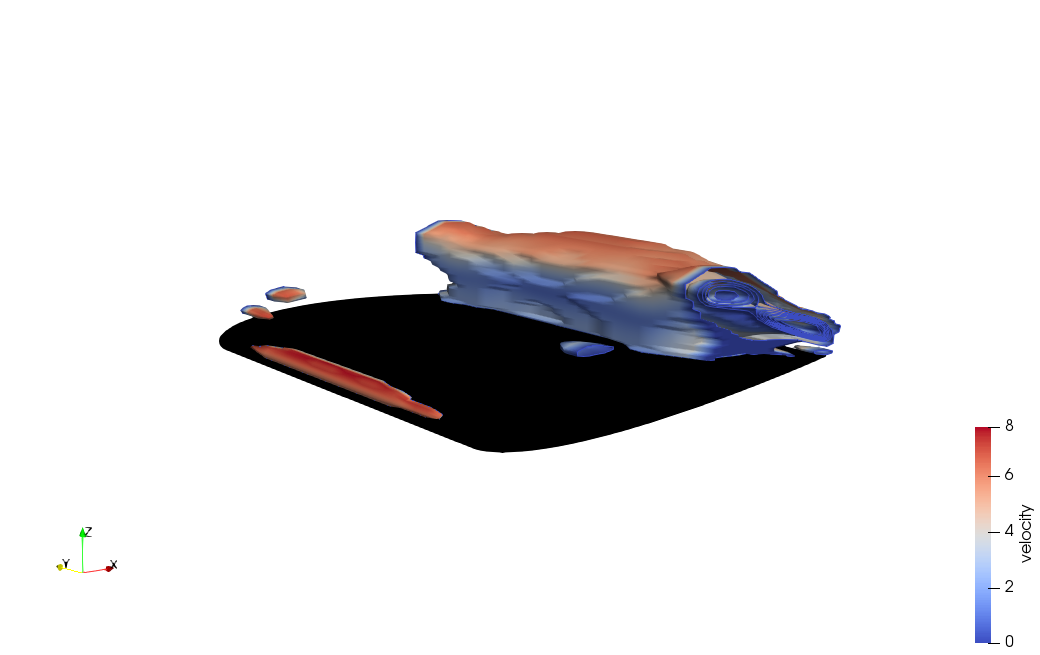
\includegraphics[width=0.3\textwidth]{AOA3Dt0.9v}}
      \caption{3D velocity distribution over a NACA0012 at different time period }
    \label{fig:fig16}
\end{figure}
U-shaped cavity occurs on the surface of the hydrofoil owing to the effects of side wall. The re-entrant flow reaches the vicinity of the cavity leading edge,and the sheet cavity lifted away from the 
hydrofoil.
As shown in figure (4.8), a re-entrant jet causes the attached sheet cavity to split along the trailing and leading edges, where the flow is attached. 
The re-entrant jet moves toward the leading edge at t=0.5s, indicating large-scale cavitation shedding.
The attached sheet cavity then collapses at a sufficiently high rate (t=0.7s), indicating that breaking has begun.
In the time interval that goes to t=0.9s, the complete shedding can be seen.
As shown in figure (4.10), the state rolls up and is carried downstream once it is vapor-filled and the re-entrant jet activates to cut the sheet cavity. 
 
\begin{figure}[H]
    \centering
    \subfloat[t=0.5 s]{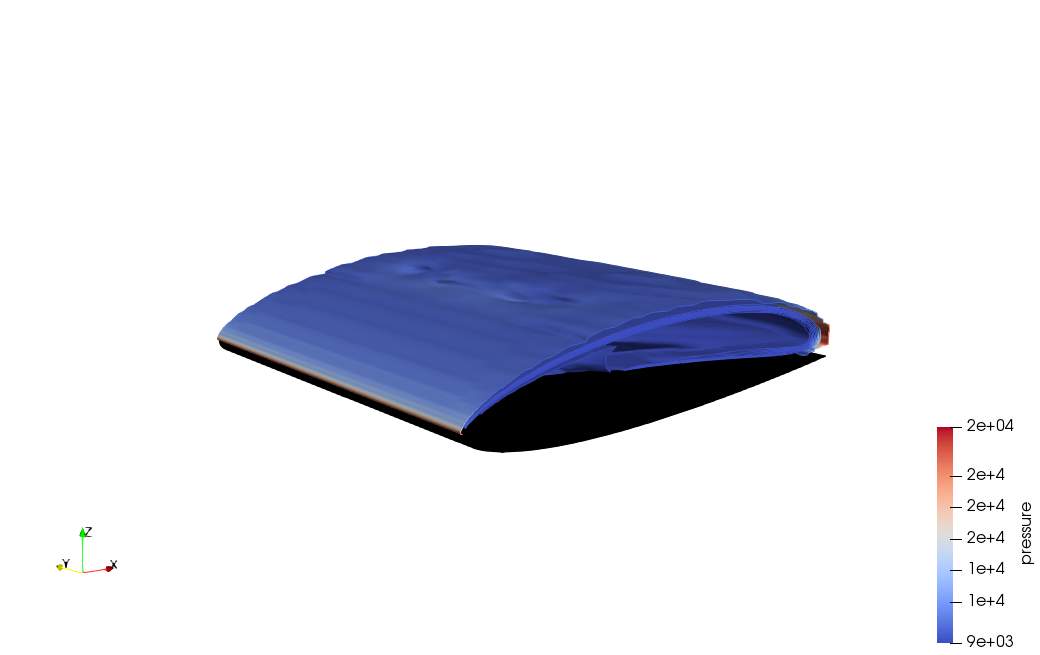
\includegraphics[width=0.3\textwidth]{AOA3Dt0.5p}}
    \qquad
  \subfloat[t=0.7 s]{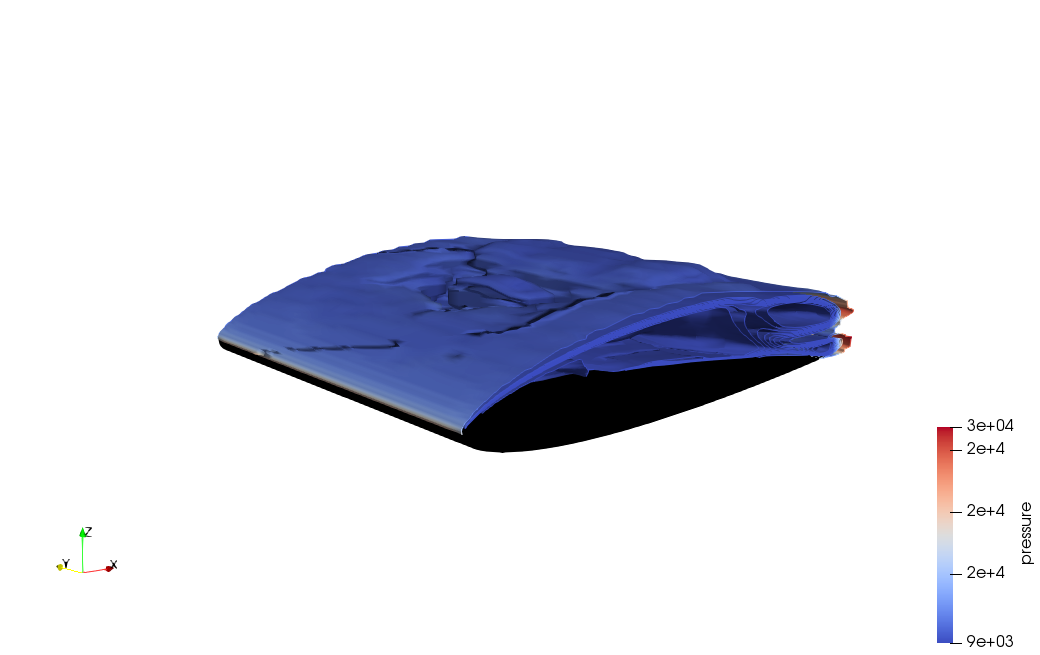
\includegraphics[width=0.3\textwidth]{AOA3Dt0.7p}}
   \qquad
  \subfloat[t=0.9 s]{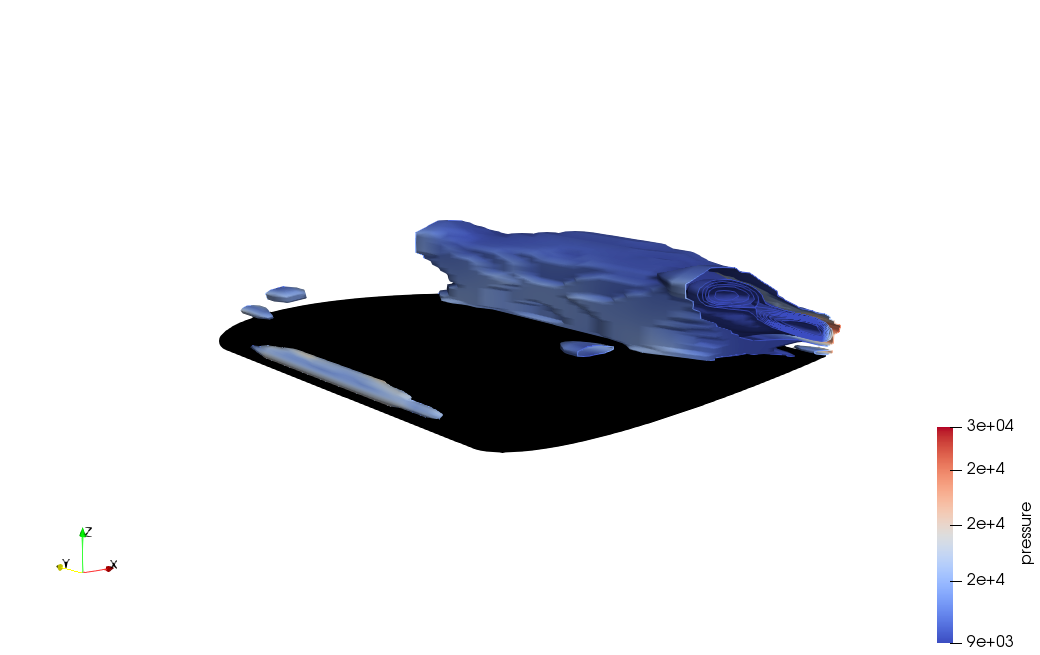
\includegraphics[width=0.3\textwidth]{AOA3Dt0.9p}}
      \caption{3D pressure distribution  over spanwise direction of NACA0012 at different time period }
    \label{fig:fig16}
\end{figure}
Figure 4.9 shows that the hydrofoil is vapor-filled at t=0.5 s, indicating that the state is in stall condition and the suction side of the hydrofoil is at saturation vapor pressure. 
\begin{figure}[H]
    \centering
    \subfloat[t=0.5 s]{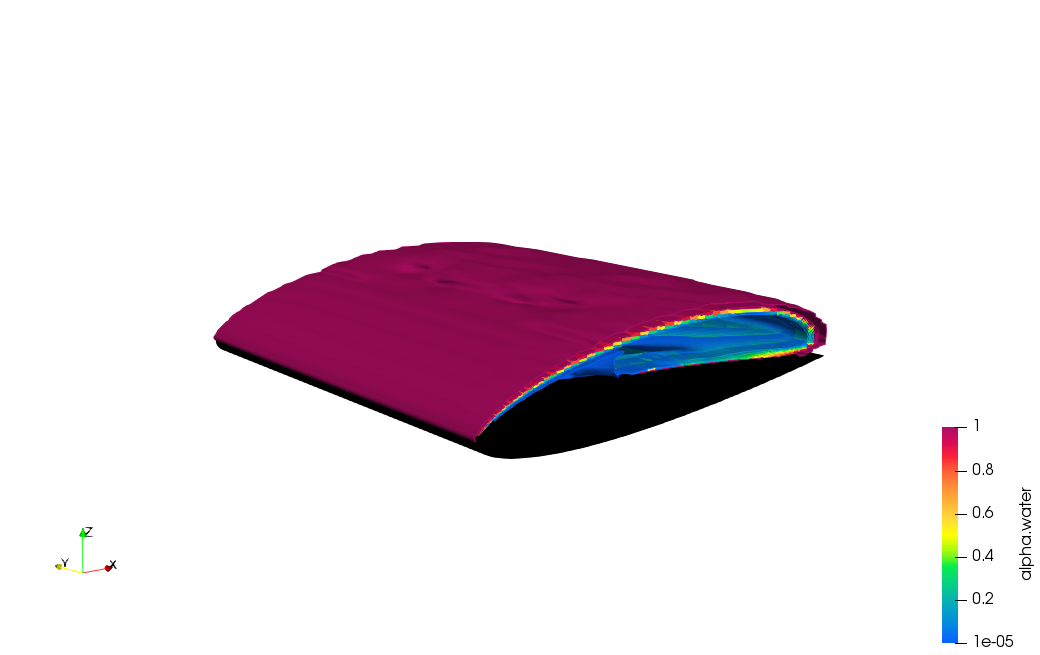
\includegraphics[width=0.3\textwidth]{AOA3Dt0.5alpha}}
    \qquad
  \subfloat[t=0.7 s]{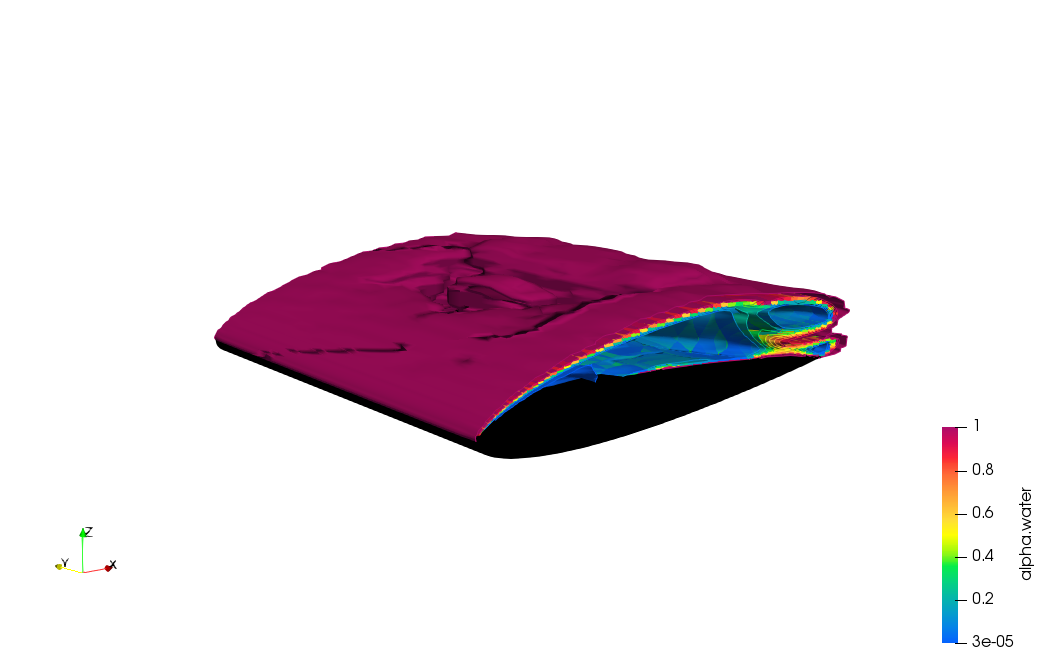
\includegraphics[width=0.3\textwidth]{AOA3Dt0.7alpha}}
   \qquad
  \subfloat[t=0.9 s]{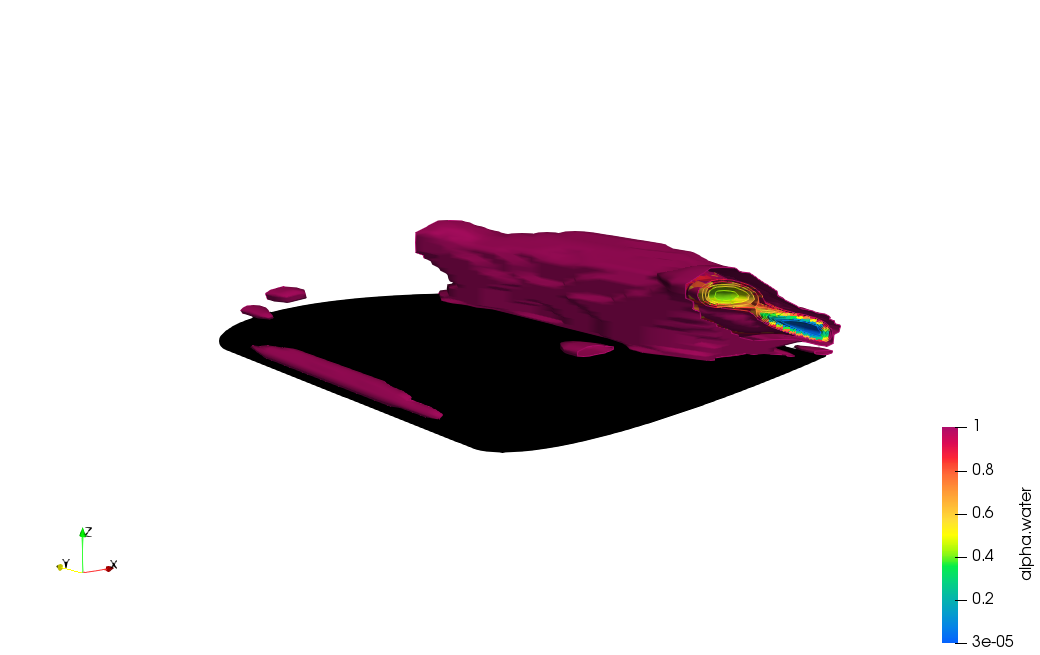
\includegraphics[width=0.3\textwidth]{AOA3Dt0.9alpha}}
      \caption{3D alpha.water distribution over spanwise direction  of NACA0012 at different time period }
    \label{fig:fig16}
\end{figure}

\begin{figure}[H]
    \centering
    \subfloat[]{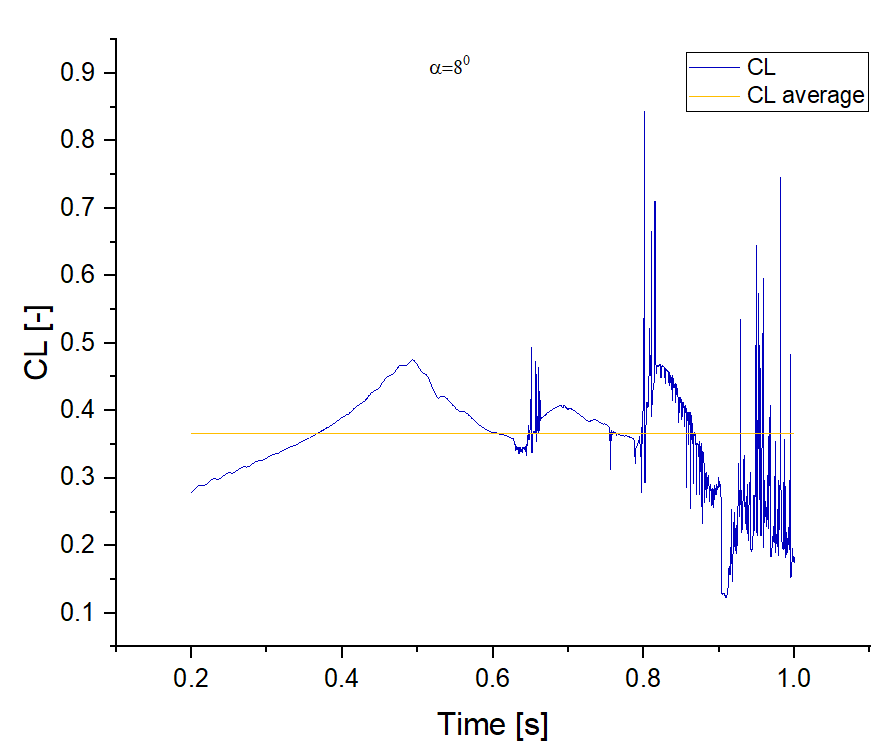
\includegraphics[width=0.3\textwidth]{AOA83DCL}}
    \qquad
  \subfloat[]{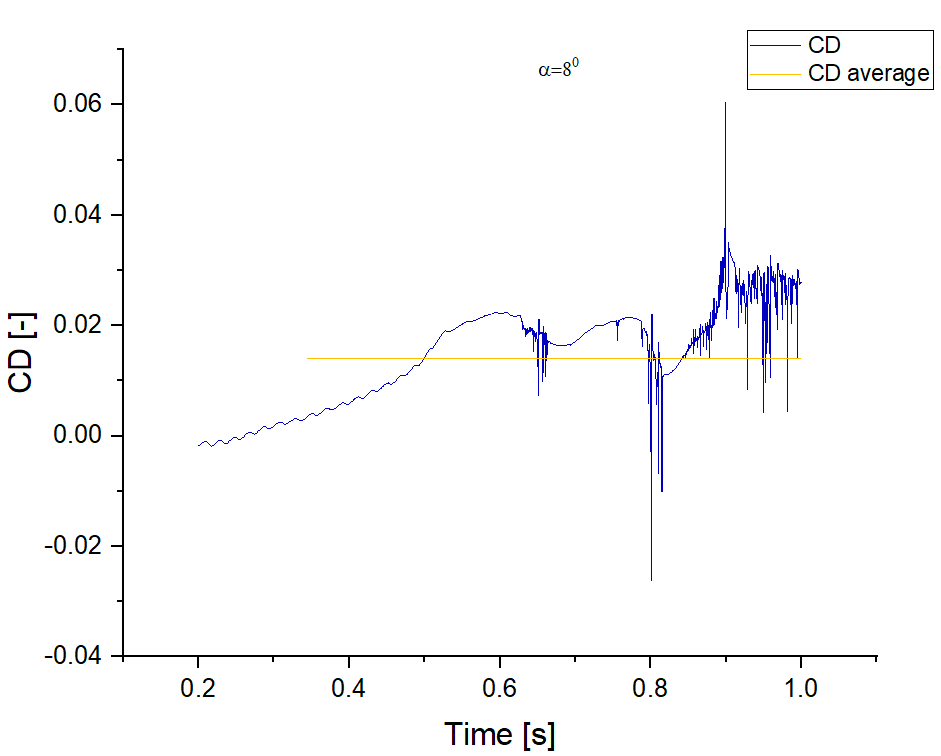
\includegraphics[width=0.3\textwidth]{AOA83DCD}}
  \caption{3D, the statistical average of force coefficient  over a NACA0012}
  \label{fig:fig16}
\end{figure}
The CL and CD of a 3D wing at $8^ {\circ}$ are 0.36 and 0.014, respectively, which is significantly less than the 2D force coefficient mentioned in the table (4.16).
The values might be also influenced by the mesh refinement, which is limited to guarantee an acceptable computational cost, in connection with the available computational power.
The mesh creation in 3D requires extra attention because it is more complicated than in 2D. However, while both the 3D and 2D models reflect the physics 
of cavitation shedding, the results are slightly inaccurate due to mesh count and turbulence model selection. 

\textbf{Comparison of numerical and experimental data}: The present work data are compared with numerical and experimental data of different authors, are given below:
\begin{table}[h]
\centering
\begin{tabular}{|l|l|l|l|l|l|l|l|l|l|l|}
\hline
\rowcolor{gray!20} ${\sigma}/{2\alpha}$& Cl Exp &Cd Exp  & Cl 1 & Cd 1 &Cl 2  &Cd 2 &Cl 3  &Cd 3  & Cl p &Cd p  \\ \hline
2.86 &0.595  & 0.061 &- &-  &-  & - &0.476  & 0.040 & 0.818 &0.059  \\ \hline
 3&0.595  &0.055  &0.580  &0.098 &0.587  &0.039  &-  &-  &0.775  &0.051  \\ \hline
 3.5&0.587  &0.045  &-  & - &0.601  &0.030  &-  & - & 0.880 &0.029 \\ \hline
4 & 0.577 &0.038  &0.576  &0.086  &0.600  &0.008  &-  & - &0.755 &0.013  \\ \hline
4.5 &0.573  &0.035  &-  &-  & - &- & - & - & 0.590 &0.021  \\ \hline
 5&0.572  &0.036  &-  &-  & - & - & - &-  &0.535  & 0.025 \\ \hline
 5.5& 0.573 & 0.036 &-  & - & - & - & - & -  &0.585  &0.023  \\ \hline
6 &0.574  & 0.033 &  &-  &-  & - & - & - & 0.543 &0.024  \\ \hline
6.5 & 0.573 & 0.035 &0.512  &0.028  & - &- & - & - & 0.505 & 0.025 \\ \hline
 7 & 0.574 & 0.035 &- & - & - & - & - &-  & 0.472 & 0.024 \\ \hline
\end{tabular}
\caption{Numerical and experimental result comparision of NACA0012 hydrofoil}
\label{fig:fig16}
\end{table}

Cl p and Cd p is "Force coefficient data of present work".
Cl Exp and Cd Exp is "Experimental data given by Takasugi \cite{Zhao2021}".
Cl 1 and Cd 1 is "Numerical data given by Ghassemi \cite{Zhao2021}".
Cl 2 and Cd2 is "Numerical data given by Karim \cite{Zhao2021}".
Cl 3 and Cd 3 is "Numerical data taken from reference \cite{Zhao2021}".\\

By comparing the numerical results of the present study with experimental data from the table (4.9), 
it appears that from 4.5 to 7 degrees, the numerical results are within 
10\% error. Conversely, a numerical result of 2.86 to 4 indicates more than 10\% error. 
This means that when dealing with higher angles of attack, special attention needs to be 
paid to the choice of turbulence model. From the reference paper \cite{Zhao2021} the numerical data for the value at 2.86 degrees is obtained by applying three different turbulence models, which are: $k- \omega$ sst, modified $k - \omega$ sst, and LES. In there, the author concluded that at higher angles of attack is better to use LES instead of RANS models because the RANS model treats the vortices of different scales equally and this affects the accuracy of the numerical value. Consequently, if we simulate flow at an angle of attack of $4^{\circ}$, it is better to use the modified $k- \omega$ sst because it gives more accurate results with cavitation cloud shedding as stated in reference \cite{Zhao2021}. Since there is no cavitation shedding when we treat flow at the $4^{\circ}$ angle of attack with $k- \omega$ SST as the turbulence model in the present work.

\chapter{Conclusions}
In the present work, k-$\omega$ sst turbulence model is used to study the steady non-cavitation flow  and 
unsteady cavitation flow with cloud shedding over a  NACA0012 hydrofoil using interFoam solver in OpenFOAM.
The cavitation flows are demonstrated and numerical result are compared with experimental result from \cite{Zhao2021}
and the following conculsions can be drawn:
\begin{itemize}
\item In the case of higher angles of attack, it needs further investigation the quantitative analysis because 
the combination of turbulence model and chosen mesh do not provide accurate quantitative results.
\item Realistically, the effect of 3D on experimental results is largely ignored in numerical simulations, 
which is why this effect shows up as a variation when comparing the numerical result with experiment results.
\item In the case of non-cavitating flows, AOA $3.2^{\circ}$ to AOA $3.8^{\circ}$, the k-$\omega$ sst model
 successfully predicts the result with less than 10 percent error when compared to experimental results. 
\item The k-$\omega$ sst model fails to replicate cloud shedding in cavitating flows, particularly between AOA $4.1^{\circ}$ and AOA $5.0^{\circ}$. 
\item Cloud shedding is observed when the angle of attack is between $5.7^{\circ}$ to $8^{\circ}$, and 
when comparing the numerical result to experimental data, it is clear that the inaccuracy is greater than 10 percent.  
\item The numerical results are typically reliable in capturing the fracture and detachment behaviors in the cavitation process. 
But RANS cannot accurately capture the features of the vortices in the flow fields at high angles of attack. 
\end{itemize}

































